\documentclass[a4paper]{article}

\usepackage[english]{babel}
\usepackage[utf8]{inputenc}
\usepackage{amsmath}
\usepackage{graphicx}
%\usepackage[colorinlistoftodos]{todonotes}
\usepackage[parfill]{parskip}
\usepackage{multirow}

\title{SSAS-E2013 Programming Assignment - Part II}
\author{Team 6:\\Christian Lyngbye, Jacob Fischer, Rasmus Greve, Ivaylo Sharkov}

\begin{document}
\maketitle

\section{Introduction}
This is the written hand-in for the second part of the programming assignment of the course. With regards to the report, we have addressed the issues presented in the feedback from the first part of the assignment. Secondly, we have incorporated the customer's requests for this assignment in our analysis and design process in order to integrate it with our existing system as seamlessly as possible.

%The report is structured... etc. TODO
We start by describing our strategy for the architecture. We try to cover the 7 touchpoints except the code review because we had trouble finding tools. 

\section{Strategy}
By defining our strategy clearly and sharing it with our users, we hope to align our strategy with our business and technology.

We start by listing our goals and afterwards we will define how and why we expect to reach them.

\begin{itemize}
\item
We hope to engage our users in a new social platform based on their interests.
\item
The brand should build trust with the users over the long term so they keep coming back.
\end{itemize}

% how
We wish to achieve our goals by providing the following features to our users:
\begin{itemize}
\item Easy signup with design that provides high quality features with as few clicks as possible.
\item Users can choose from a long list of social hobbies and find others with the same interests.
%\item Full data ownership: All data is owned by the users and should be easy to export and reuse.
\end{itemize}

\subsection{Risk Analysis and Management}
The business context is an application developed by a small enterprise with public customers with no contract of any sort. We provide a rudimentary service level agreement though there is no consequences if it is compromised. Most of the analysis is based on experience from using similar applications or our projections of how prospective interviewees would answer our questions.
\subsubsection{Business Goals}
We have decided on the following goals as paramount to our business operation with the web application. If any of these are not met, we consider it a severe threat to the integrity of our business.

\begin{table}[h!]
	\begin{tabular}{|p{10cm}|l|}
		\hline
		\textbf{Business Goal} & \textbf{Rank} \\ \hline
		The server must provide 99.95\% uptime   & \textbf{M} \\ \hline
		Sensitive user data is never compromised & \textbf{H} \\ \hline
		The application should be improved gradually by releasing new versions often & \textbf{L} \\ \hline
		Application must be live by October 4th 2013 &	\textbf{H}\\ \hline
		The application should be usable by a novice computer user on small screens (smartphones) as well as desktops & \textbf{M}\\ \hline
	\end{tabular}
	\caption{Business goals for our project. The goals are ranked with letters where L: low, M: medium and H: high}
	\label{tab:business_goals}
\end{table}



\subsubsection{Business Risks}
We have analyzed the business risks of the project and determined their impact which we have imagined as they would be for a small size enterprise.
\begin{table}[h!]
\begin{tabular}{| p{4cm} | p{3cm} | l | p{3cm} |}
\hline
\textbf{Business Risk} & \textbf{Indicators} & \textbf{Likelihood} & \textbf{Impact} \\ \hline
Data loss & Reports of service outage & L & Loss of potential users\\\hline
A user is subject to social engineering & Reports of peculiar activity & H & Damage to brand \\\hline
Vulnerabilities in the system & High amount of breaches & H & Unintended downtime and higher development costs \\\hline
Application delayed & System features are implemented late & M & Late return on investment \\\hline
\end{tabular}
\end{table}


\subsubsection{Technical Risks}
The technical risks are characterized by their probability and effect on the system in table \ref{tab:risk_analysis}. We have also identified risks in making the system too secure.

\begin{table}[h!]
	\begin{tabular}{| l | p{3cm} | l | l |}
		\hline
		\textbf{Risk} & \textbf{Indicator} & \textbf{L} & \textbf{C}  \\ \hline
        User login bruteforcing & Repeated login attempts in logs & M & 6 \\ \hline
        %TR5 & SQL injections & 80\% & 9 & Prepared statements and input sanitization \\ \hline
        User session hijacking & Reports from users of peculiar behavior & M & 4 \\ \hline
        Old libraries and platforms provide an easy target & Unsupported software & H & 9 \\\hline
        Hardware failure & Reports of downtime & L & 5 \\ \hline
        Security is not part of system architecture design & Unsecure design & M & 7 \\ \hline
		Security safeguards slows down user experience & Too many interactions & L & 3
		\\ \hline
	\end{tabular}
	\caption{Risk analysis for the social network system with mitigation strategies. L: Likelihood that it will occur. C: Consequences on a scale from 1 to 10}
	\label{tab:risk_analysis}
\end{table}



In table \ref{tab:goal_to_risk_relationship} the business and technical risks are synthesized. The technical risks are from table \ref{tab:risk_analysis}.

\begin{table}[h!]
	\begin{tabular}{| p{4cm} | p{4cm}| p{4cm} |}
    \hline
   	\textbf{Business goals} & \textbf{Business Risk} & \textbf{Technical risk} \\ \hline
    \multirow{3}{4cm}{Sensitive user data is never compromised} & \multirow{3}{4cm}{Vulnerability in the system} & User credentials bruteforce \\ & & Old libraries and platforms provide an easy target \\ & & User session hijacking \\ \hline
    The server must provide 99.95\% uptime & Data loss &  Hardware failure \\ \hline
    %\multirow{4}{4cm}{The web server is breached at most twice throughout the project period} & \multirow{4}{4cm}{Vulnerabilities in the system} & TR5 & SQL injection \\ & & TR8 & Replay attack \\ & & TR9 & Cross-site request forgery \\ & & TR12 & Cross-site scripting (XSS) \\ \hline    
    Application must be live by October 4th 2013 & Application delayed &  Security is not part of system architecture design \\ \hline
    The application should be usable by a novice computer user on small screens (smartphones) as well as desktops & A user is subject to social engineering & Security safeguards slows down user experience \\ \hline
    \end{tabular}
    \caption{Goal-to-risk relationship table.}
	\label{tab:goal_to_risk_relationship}
\end{table}



\subsubsection{Mitigations}
We have ranked the risks and provide our proposals for mitigation.
\textbf{Vulnerability in the system}
Use supported third party libraries to keep all parts of the software secure to avoid the compromise of sensitive user data by Securing the Weakest Link.


By assigning clients user credentials we can identify them and separate them into different roles that we might need and do \textbf{Separation of Privilege}.

\textbf{Data loss}
We do backups of the database and encrypt it.

\textbf{Application delayed}
Having a planned milestone gives an idea of what it is possible to do.
Decreasing the scope to something manageable helps as well.

\textbf{A user is subject to social engineering}
Providing warnings to users.

% why
%\begin{itemize}
%\item Reluctance to Trust
%\item Securing the Weakest Link
%\item Failing Securely
%\item Least Privilege
%\item Separation of Privilege
%By assigning clients user credentials we can identify them and separate them into different roles that we might need.
%\item Promoting Privacy
%\end{itemize}
%Confidentiality, Integrity, Availability

\section{System Specification}
In accordance with the project description, we have defined our system as a web application where students can form friendly or romantic relationships with other students. The application should furthermore support administrative users, who are able to modify certain aspects of the system from a client's perspective. These requirements derive from the user stories presented in the project description. Since we are at part two of the project, there have so far been two such sets of requests from the "customer".

We have considered each of these user stories and made corresponding use cases for the system, leading to functional requirements. Some of the user stories have related instead to non-functional requirements, and some again to security requirements.

In addition, we have specified a number of abuse cases, constituting a security-related counterpart to the use cases. Based on these, we have derived additional functional, non-functional and security requirements. Not all abuse cases have had equal impact on the final specification, as we have had to keep in mind the strategic prioritizations outlined in the Risk Management section.

\subsection{Use cases}
\begin{itemize}
\item A student views his own information
\item A student edits his own information
\item A student chooses what information to share
\item A student views another student’s information
\item A student forms a friendly or romantic relationship with another student
\item A student sends a "hug" to mutual a friend or romance
\item An administrator creates a new user
\item An administrator deletes an existing user
\item An administrator views the information of a user
\end{itemize}

\subsection{Abuse cases}
\begin{itemize}
\item A malicious user runs arbitrary queries on the database by submitting SQL code through an input field
\item A malicious user fills the system with irrelevant data by automatically creating multiple user profiles with a self-repeating script
\item An unauthorized third party is picking up a user's traffic by listening on the same network the user is connected from
	\begin{itemize}
		\item The third party gains access to sensitive user data against the regulations of the privacy policy
		\item The third party gains access to the user's session ID, allowing the intruder to impersonate the user when communicating with the application
	\end{itemize}
\item A person with access to an administrator's credentials wreaks havoc on the system by deleting multiple user profiles
\end{itemize}

\subsection{Functional Requirements}
Most of the following functional requirements are derived from the use cases, to support the functionality that the customer has requested in the project description. A few requirements have been added and/or modified based on the abuse cases, however, and these are marked with a star (*) and mentioned here.

* In order to prevent an intruder who has hijacked a user's session ID from tampering with the user profile itself, we require users to re-enter their password whenever they submit changes to their profile data.

** In order to prevent people with access to an administrator's credentials from destroying user data in the system, an administrator is only able to suspend (and not delete, as per the use case) user profiles. Other administrators will then be able to restore the profile, in the case of a mistake. We feel that this is a good compromise, which does not stray too far from the original use case.
\begin{itemize}
\item A database model supporting users with the following data represented:
  \begin{itemize}
  \item User
      \begin{itemize}
      \item Username (this is necessary as the customer wants both proper name and email to be private information)
      \item Password
      \item Email
      \item First name
      \item Last name
      \end{itemize}
  \item Hobbies
  \item Friends/romances
  \end{itemize}
\item CRUD for users
	\begin{itemize}
    \item Users should be able to view their own data
    \item Users should be able to view other users' data, filtered depending on their relationship with the given user
    \item Users should be able to edit their own data upon re-entry of their password *
    \item Admins should be able to create new users
    \item Admins should be able to suspend and restore user profiles **
    \end{itemize}
\item User authentication
\item Admin authorization
\item Browse functionality for finding other users
\end{itemize}

\subsection{Non-functional requirements}
The following is our non-functional requirements to the system. These are derived from our business goals, one of which relates to uptime. Another of our business goals is to employ immediate mitigation against any attack we might be subject to throughout the project period. To this end, it is imperative that we run an active logging framework.
\begin{itemize}
\item The application is available through an HTTP connection 99.95\% of the time
\item A logging framework is enabled that allows the team to identify the underlying causes of any breaches that may occur
\end{itemize}

\subsection{Security Requirements}
Based on the prioritizations of the Risk Management section, as well as the previously listed abuse cases, we have derived the following security requirements to our application.

We do not require the application to run through a secure connection, as although it would provide good protection against abusive users sniffing packages on an open network, we consider it a too extensive task to implement within the scope of the project, having prioritized other things. Instead, as previously mentioned, we have modified our functional requirements to mitigate this particular abuse through alternative means.
\begin{itemize}
\item A firewall blocks requests on all ports but port 80 (HTTP) and port 6666 (SSH)
\item Database access credentials are never stored in any source code repository
\item The database is always accessed in a manner that protects against SQL injection
\item The application guards against cross-site scripting
\end{itemize}

\section{Architecture}

Our production server runs Linux and provides the access control for users' access to the file system.

We have attempted to restrict privilege given on our server so users are given 
\textbf{Least Privilege} as possible to the file system. We have disabled remote login for the root user and every member of the team has a user that is in a superuser group. The application server and database runs each with their respective user that is only used for that process. However we need to give root access to the application server because it needs to run on port 80.


Our database is our most valuable asset and therefore we wish to protect it. The database user/role for the database creation is different from the user that is used by the application server. By applying this practice we give the application the least possible privilege to the database to protect our database from being dropped. Furthermore we store the username and password to the database on the server and we don't share the username and password in our VCS according to the principle of \textbf{Reluctance to Trust} since we don't trust the confidentiality of our VCS.

Our application authorizes users in order to determine the privilege for access to user stories like pages that a user has.

We replaced the error page in order to \textbf{Fail Securely}.
\begin{figure}[h!]
\centering
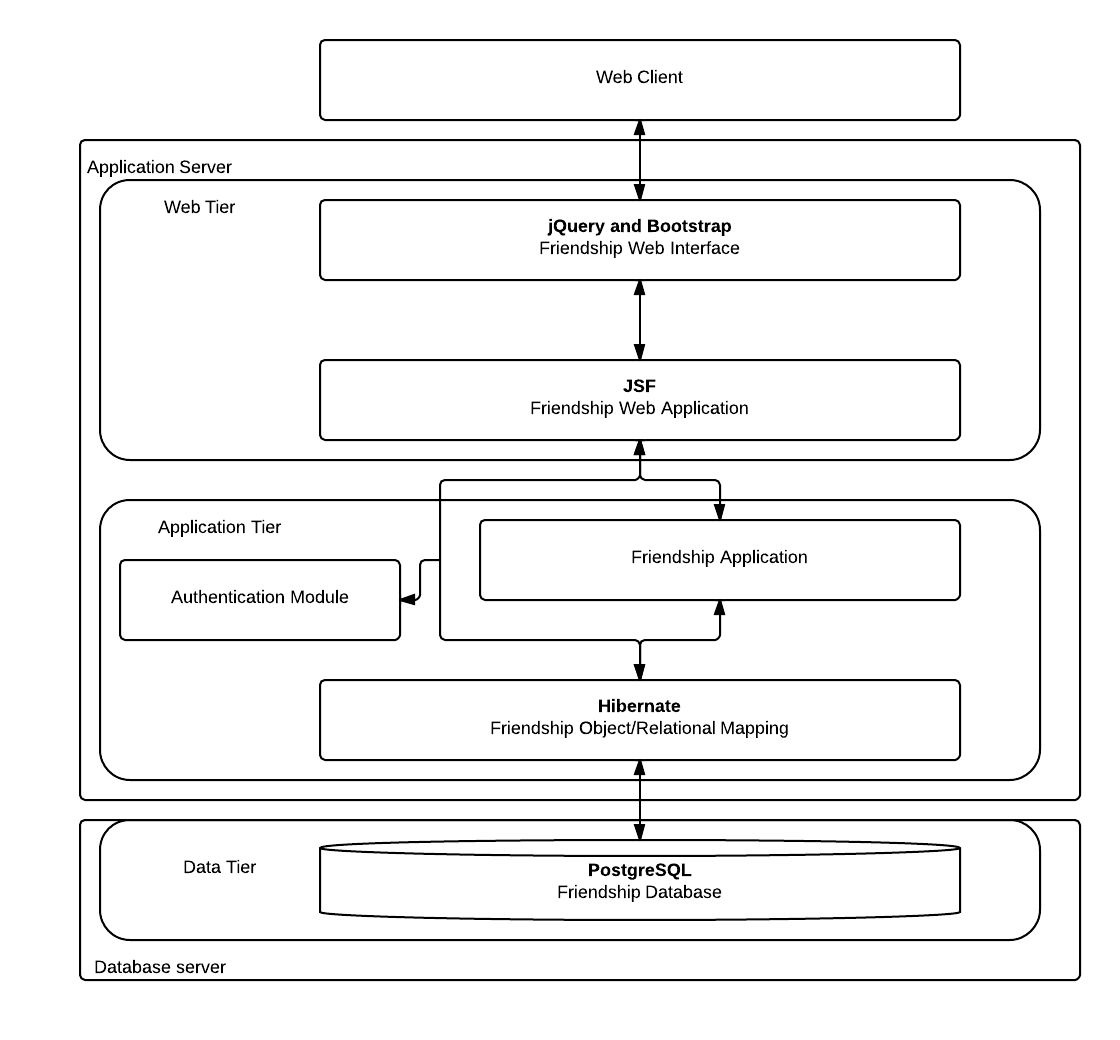
\includegraphics[scale=0.3]{ForestView}
\caption{Forest View diagram}
\label{fig:forest_view}
\end{figure}


\subsection{ER modelling}


\begin{figure}[h!]
\centering
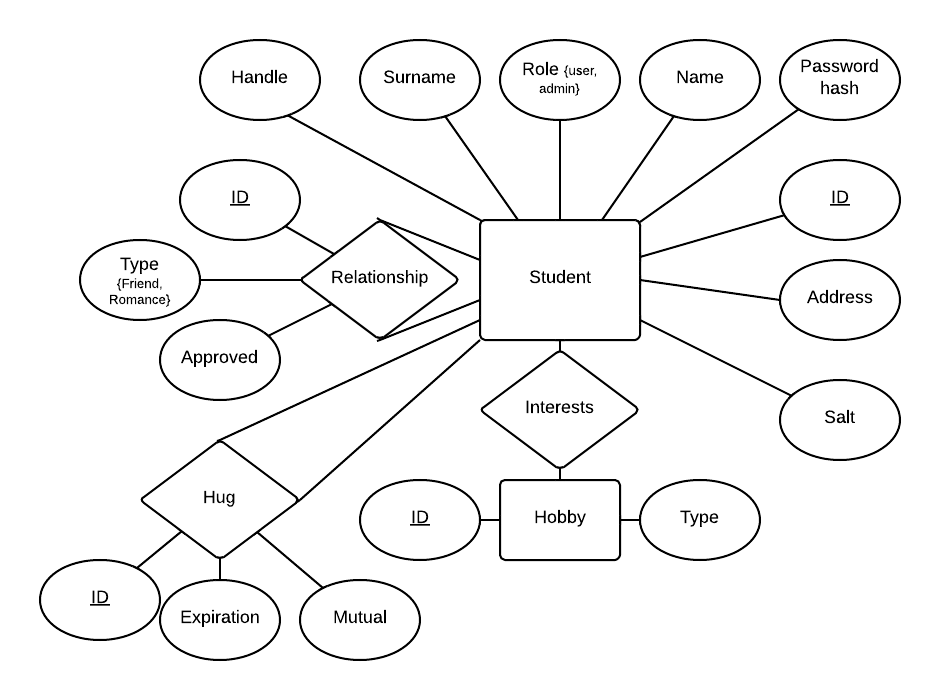
\includegraphics[scale=0.5]{ER}
\caption{Entity relationship diagram of our data-model}
\label{fig:er_diagram}
\end{figure}



\subsection{Choice of Technology}
\subsubsection{Frameworks and Technologies}
The following is a list of all the frameworks and technologies we have decided to use, with a short justification for each.
\begin{itemize}
\item \textbf{JSF2} is the recommended dynamic web page technology for this course, which makes help more readily available. In addition, we are all fairly experienced with Java, and one person on the team has prior experience with JSF. It provides protection against XSS and CSRF. \textbf{(TODO: Ensure that we actually do use JSF2 and not 1.21)}
\item \textbf{Tomcat 7} is a web application server, as with the above, is the recommended server technology.
\item \textbf{UFW}, the Uncomplicated Firewall, is a straightforward firewall implementation for Linux.
\item \textbf{Hibernate} is a library that provides ORM and can encapsulate database access in transactions and maps objects to relations.
\item \textbf{PostgreSQL} is our chosen database technology. Among other things, it provides fine-grained user access control.
\item \textbf{JUnit and Selenium with Selenide} for testing our application. JUnit provides a unit-testing framework for Java, which Selenium integrates with. Selenide is a framework for running tests for a web application through the browser.
\end{itemize}


\textbf{SHA-256} algorithm for hashing our users' passwords. It is generally regarded as a considerably secure hashing algorithm.
We also use a randomly generated 4 character salt for every user.

\subsubsection{Project Tools}
We have chosen to use the following tools to assist us in our project process.
\begin{itemize}
\item \textbf{Git} is our chosen tool for source control, since it is easy to use and gets the job done, and Github is a decent platform for hosting source code on.
\item \textbf{Google Docs} is what we use for taking notes and making on-the-fly documents, spreadsheets or presentations that we might need throughout the project. It is very easy to share things here, but the text processing tool is not that powerful, so it is not where we write our report.
\end{itemize}


\section{Testing}

\subsection{Test plan}

\subsection{Tools and Frameworks}
Testing is essential in order to build secure and functional software systems. To thoroughly test our system we have decided to use two testing strategies; system tests and unit tests.

A testing tool we found fitting to use for system tests is Selenium with JUnit. Selenium allows us to script test cases which input data and submit forms on the webservice.

\subsection{System Test Cases (Black-box Test)}

\begin{itemize}
\item Login
\item SQL injection in input
\item Access to unauthorized pages
\item Creating user
\item Renewing password
\end{itemize}

\subsection{Penetration Testing}
The application protects against the following:
\begin{enumerate}
\item{SQL injections}
\item{XSS attacks}
%\item{Login bruteforcing}
%\item{Admin subject to social engineering}
\end{enumerate}

We have chosen this prioritization of threats by looking at the probability and consequenses of each of them as well as estimating how complicated it is to implement the mitigation strategy.

SQL injections and XSS attacks are relatively easy to protect against in our setup as the tools we use, prevent these kinds of attacks. Hibernate, which we use for ORM, renders any SQL injection attempt useless, and JSF protects against XSS attacks.
%TODO: Does JSF protect against XSS attacks?
\section{Hacking}
\subsection{Plans and ideas}
In this section we describe plans and ideas for hacks and attacks that we haven't (yet) conducted.
\subsubsection{Social engineering attack}
A social engineering attack requires some knowledge and analysis of the setting, system and people you want to attack.

The setting at hand is that we are among a set of teams all implementing and trying to secure a webservice which must be "handed in" and shown off to a teacher and possibly the TA. This implies that the people in the teams all trust both the teacher and the TA. We have observed that most of us do not remember the name of the TA off the top of our heads and need to look it up on the course blog.
We can use this knowledge to make a broad social engineering attack on all other groups attempting to obtain confidential information such as usernames and passwords for admin accounts.

The idea is to send an email to the entire class that looks and sounds official and says that it is from ``The TA of System Architecture and Security F2013". We assume that the students are not aware of the name of our TA and that they will trust that if we claim to be him in the email, they will believe us. The email will contain a request for login information to their webservice for an admin account that we need in order to evaluate the teams' progress.

A requirement for this attack to work is that we send the email before (if) the teacher or TA asks for this information from the groups. We plan on sending the email on the 4th of October.


\textbf{Team 1}

%Inserted the following as username and password in login form:
%\begin{verbatim}
%' OR 1 = 1;--
%\end{verbatim}
%This resulted in a 502 error followed by errorcode 500 responses on following %attempts at reaching the website.
%In order to submit the form the in-browser email verification had to be disabled %(achieved by editing the DOM such that type="email" became type="text")


\section{Discussion}
\subsection{Problems}
\subsection{Deployment}

\subsection{...}


\section{Conclusion}

\newpage
\section{Appendix}
\subsection{Log file}
\begin{verbatim}
Nov 1, 2013 9:40:45 AM dk.itu.ssase.hb.beans.LoginBean validateUser
INFO: Authenticated user admin
Nov 1, 2013 9:40:51 AM dk.itu.ssase.hb.listener.AuthPhaseListener afterPhase
INFO: Authorized user
Nov 1, 2013 9:40:51 AM dk.itu.ssase.hb.beans.StudentBean addHobby
INFO: Hobby id: 2
\end{verbatim}

\subsection{Test reports}
\begin{verbatim}
-------------------------------------------------------
 T E S T S
-------------------------------------------------------
Running dk.itu.ssase.test.LoginTest
Tests run: 2, Failures: 0, Errors: 0, Skipped: 0, Time elapsed: 12.814 sec
Running dk.itu.ssase.test.SignupTest
Tests run: 1, Failures: 0, Errors: 0, Skipped: 0, Time elapsed: 1.45 sec

Results :

Tests run: 3, Failures: 0, Errors: 0, Skipped: 0

------------------------------------------------------------------------
BUILD SUCCESS
------------------------------------------------------------------------
\end{verbatim}

\textbf{Team contract}

The team consists of the following four members:
\begin{itemize}
\item{Jacob Fisher (jaco@itu.dk)}
\item{Christian Lyngbye (clyn@itu.dk)}
\item{Ivaylo Sharkov (isha@itu.dk)}
\item{Rasmus Greve (ragr@itu.dk)}
\end{itemize}
Our expectations of the project is to create a working product with a report meeting all requirements at the right deadlines. We expect to get at least a passing grade and strive towards getting a 10 or 12 at the exam.

We agree on doing project work at least once a week, usually on fridays from 10am to around 2-4pm depending on the amount of work to be done and the deadlines.

Three group members have an exam in week 42. After this, we should be able to meet some Thursdays as well.

Rasmus is having a baby in the end of October and will not be able to do group work on site at ITU in a couple of weeks after this time. He will do work from home and keep in touch with the group via email and instant messaging.

\textbf{Week 37 (13/09/2013)}

Today we created our course log and a git repository.
Jacob retrieved information for our server slice.

We decided on which technologies we were going to use:
We would use the programming language Java and create a Web Application that would use JSF and ORM to map objects to a relational database.

We chose to user a Tomcat server as the application server.

For source control management we have shared a private repository on Github.

We made some agreements in the group regarding collaborative tools.
We chose to use LaTeX to write the report and hosted it on writeLaTeX.
Google Drive for file sharing.
Facebook for communicating outside of the university.

On the server slice we set up a firewall to filter all ports except 6666 which we use for SSH.
We disallowed root access to SSH.
In order to run the application on the server we downloaded and installed: Java JDK, Apache Tomcat and Git.
We discussed how to deploy to the server and considered building the application locally on the server.

We made an initial draft of user stories and requirements for our system.


\textbf{Week 38 (20/09/2013)}

As an experiment Christian installed PostgreSQL on the server slice and it was proved to work so we chose to use it. 
Christian scanned all team servers with nmap and found some differences in solutions e.g. turning ping responses off and closed ports.
Added an example Netbeans project with JSF and started working on connecting to the database.
Rasmus designed the database diagram created an initial creation script for the database.

Ivaylo analyzed the risks.

Planned to do code review and architectural risk analysis.


\textbf{Week 39 (27/09/2013)}

This week we began work on the project report by determining which chapters we need. Jacob started writing the choices of technology chapter and the introductory chapters.

The goal and risk analysis was elaborated on and importet into the report LaTeX document.

We discussed and planned a social engineering attack targeted at all the other groups involving impersonating the TA in an email. We agreed that it was still too early in the process to perform this attack since most teams would be unlikely to have a working webservice to which we could gain access.

\textbf{Week 40 (04/10/2013)}

Ivaylo was sick today and was unable to do group work.

Christian made some refactoring in the codebase requiring the rest of the team to reimport the project into NetBeans.
This refactoring included renaming the project and introducing the Selenide testing framework and a few sample test cases to be elaborated on later. The system is now called ``FriendSpace''.

Rasmus spent a bit of time styling the webpages using Twitter Bootstrap. Jacob drew a logo to make the visual expression of the webpages more appealing.

The system was deployed to the webserver on port 80 which was opened. Accessing the root of the server redirects the user to /ssase13.

Furthermore, the team spent a lot of time throughout the day finishing up the first draft of the report for the first hand-in.


\textbf{Week 41 (11/10/2013)}


\textbf{Week 42 (18/10/2013)}


\textbf{Week 43 (25/10/2013)}

Worked on Sins presentation about Race Conditions. This led to some improvements of our code.

\textbf{Week 44 (01/11/2013)}
\textbf{Week 45 (08/11/2013)}

Reorganized the report into distinct sections.
Divided work between us to help organize.

\textbf{Week 46 (15/11/2013)}

Implemented friend requests.
Rewrote risk analysis to use the book structure.

\end{document}
